\documentclass[12pt,a4paper]{report}
\usepackage[latin1]{inputenc}
\usepackage{amsmath}
\usepackage{amsfonts}
\usepackage{amssymb}
\usepackage{subfig}
\usepackage{graphicx}
\usepackage{listings}
\usepackage{colortbl}
\usepackage{longtable}
\usepackage[final]{pdfpages}
\usepackage{float}
\author{Lauren Frazier}
\title{Evaluation of Gesture-Based Controls for Robotic Systems}
\begin{document}

\begin{titlepage}
\begin{center}
{ \Large EVALUATION OF GESTURE-BASED CONTROLS FOR ROBOTIC SYSTEMS } \\[1cm]

{\Large Lauren E. Frazier} \\[1cm]

{A THESIS} \\[1cm]

in \\[1cm]

{\Large Computer and Information Science}\\[1.5cm]

Presented to the Faculties of the University of Pennsylvania in Partial Fulfillment of the Requirements for the Degree of Master of Science in Engineering\\[1cm]

2012 \\[2.5cm]

\rule{0.6\linewidth}{0.1mm} \\
Norman I. Badler\\
Supervisor of Thesis \\[2.5cm]

\rule{0.6\linewidth}{0.1mm} \\
Jianbo Shi\\
Graduate Group Chairperson
\end{center}
\end{titlepage}


%%%%%%%%%%%%%%%%%%%%%%% TODO LIST %%%%%%%%%%%%%%%%%%%%%%%%%%
%\newcommand{\todo}[1]{
%    \addcontentsline{tdo}{todo}{\protect{#1}}
%    \marginpar{#1}
%}
%
%\makeatletter \newcommand \listoftodos{\section*{Todo list} \@starttoc{tdo}}
%  \newcommand\l@todo[2]
%    {\par\noindent \textit{#2}, \parbox{10cm}{#1}\par} \makeatother
    
    
%\listoftodos
%%%%%%%%%%%%%%%%%%%%% END TODO LIST %%%%%%%%%%%%%%%%%%%%%%%%%

\setcounter{page}{1}
\pagenumbering{roman}
\tableofcontents
\listoftables
\listoffigures

\chapter*{Acknowledgements}
\addcontentsline{toc}{chapter}{Acknowledgements}
These are acknowledgements.

\chapter*{Abstract}
\addcontentsline{toc}{chapter}{Abstract}
Robotic control systems are becoming more common, especially in the military, and there is a growing need for better control interface. Arm and hand gestures are typical human forms of communication, so applying that to a robotic control system can yield a more intuitive system. With military applications, there are lives at stake, so having the most efficient, intuitive control system can make a large difference in the success of a mission and the safety of the soldiers involved. 
The work in \cite{Varcholik_Barber_Nicholson_2008} describes a gesture based control system that uses the Nintendo Wiimote to determine arm/hand gestures and control a robot. I propose to create a gesture based system using a smartphone and conduct an experiment similar to the work in \cite{Varcholik_Barber_Nicholson_2008}, collecting survey data from the participants on the the effectiveness and ease of use of each system. This thesis aims to test the effectiveness/ease of use of smartphone gesture-based robotic control systems vs. traditional control systems.

\chapter{Introduction}
\pagestyle{headings}
\setcounter{page}{1}
\pagenumbering{arabic}

The need for human-robot interfaces is increasing rapidly. The military has already begun using unmanned vehicles in several different arenas (air, ground, water). In order to develop the most efficient human-robot interface, we turned to a traditional form of human-human communication, arm and hand gestures. Arm and hand gestures are typical human forms of communication, so applying that to a robotic control system can yield a more intuitive system. With military applications, there are lives at stake, so having the most efficient, intuitive control system can make a large difference in critical moments and improve the safety of those involved. A more intuitive system will also reduce the training time and expenses for the operators of the vehicle.

The work in \cite{Varcholik_Barber_Nicholson_2008} describes a gesture based control system that uses the Nintendo Wiimote to determine arm/hand gestures and control a robot. They then conducted a study where subjects used Wiimote gesture system and a more standard system and filled out a survey to indicate how effective the Wiimote system was as compared to the standard control system for the robot.

I propose a gesture based system using a smartphone and conducted a human factors experiment similar to \cite{Varcholik_Barber_Nicholson_2008}. The system uses a Samsung Galaxy S II phone for the gesture-based input, a tilt-based controller, and a touch screen D-Pad controller, and a Microsoft XBOX 360 controller for the more traditional input. Subjects used each of the four controls in a random order to guide an iRobot Roomba vacuum cleaner through a short time trial course. The raw data (video and observations during the time trials) was analyzed with metrics like the time required to complete the course, number of times the subject went outside the course boundaries, number of times the subject acknowledged making a mistake, etc. After the experiment is complete, subjects also filled out a survey, and both sets of data were used to determine which control scheme is more effective and intuitive. 

This thesis aims to test both the perceived and actual effectiveness and ease of use of smartphone gesture-based robotic control systems vs. traditional control systems.

% Contributions
%This paper makes the following contributions:
%(1)  Introduces a gesture based control system using a smartphone.
%(2)  Provides data showing physical reactions to different control systems in addition to survey results after the experiment.
This thesis introduces an inexpensive gesture based control system that uses commercial, off the shelf hardware (an Android smartphone and a Roomba vacuum cleaner). It also provides data showing both subjects' objective performance and their perceived experience with each controller.

% Document articulation
The remainder of this thesis is organized as follows. In the next chapter, I present a taxonomy of related work. Chapter 3 provides implementation details for the different controls. Chapter 4 describes the design of the human factors experiment, including choice of hardware, track design, experimental procedure, and the questionnaire. In Chapter 5, I analyze and discuss the results of the experiment. Chapter 6 provides the conclusion and a brief summary. 

\chapter{Related Work}
There is a large body of work about robotic control systems that led up to this point.  The work in \cite{Varcholik_Barber_Nicholson_2008} references three papers in human-robot interaction: \cite{Waldherr}, \cite{Rogalla}, and \cite{Guo}. The work in \cite{Waldherr} presents a computer vision based approach to human-robot communication where the computation is done onboard the robot. The work in \cite{Rogalla} presents work on using both gestures and speech. The speech commands are used to augment and clarify the hand gesture commands. The work in \cite{Guo} presents a system for using the Wiimote to control a robotic dog, even showing that the Wiimote
outperformed the standard computer keyboard.

The work in \cite{Waldherr} takes a computer vision based approach to gesture recognition. It explores several methods like template-based matching and neural networks. It is derived from several other vision-based works, like \cite{Kortenkamp}, which used optical flow to recognize up to 6 gestures, and \cite{Kahn}, which recognizes pointing gestures using feature maps and the color of the user's clothing.

The work presented in \cite{Rogalla} integrates speech recognition into the system, but it also uses a computer vision based gesture recognizer. It draws from \cite{Kestler}, which recognizes static hand gestures from still photos, and CORA, a robotic assistant that uses speech and deictic gestures to execute commands (ex. ``Turn and face me").

The work in \cite{Guo} uses a Wiimote to control a Sony AIBO robotic dog. It describes a guide to designing effective human-robot interface \cite{GoodrichOlsen}. It also describes \cite{YancoDrury}, which classifies and details robotic control schemes and defines terminology related to HRI. The work in \cite{YancoDrury} defines the autonomy level of a robot as the percentage of the time that the robot carries out a task on its own (as opposed to intervention from the operator). Like \cite{Guo}, this paper deals with a robot with a low autonomy level.

\section*{Comparison to Prior Work}
While this paper has most of its origin in \cite{Varcholik_Barber_Nicholson_2008}, there are a few differences. The work in \cite{Varcholik_Barber_Nicholson_2008} uses a Nintendo Wiimote to control the actions of the robot, rather than a smartphone or XBOX controller. In the case of the smartphone, computation of gestures is performed on the phone, rather than on an intermediate computer. Like the work presented in \cite{Varcholik_Barber_Nicholson_2008}, this system uses the movement of the controller, rather than a computer vision system to observe the user. This gives the added benefit that the user can move while controlling the robot without getting out of range of a camera. The work in \cite{Varcholik_Barber_Nicholson_2008} uses an algorithm based on the 2D gesture recognition presented in \cite{Rubine}, while my gesture recognition system is based on \cite{TaKG} and uses Dynamic Time Warping to classify gestures. 

\chapter{Implementation of Control Systems}
In this chapter I will describe the implementation of the four control systems used in the experiment. First, I describe the ``standard" XBOX 360 controller setup, then the application used for the D-Pad and tilt controllers, and finally the gesture-based control application.

The robot in question is an iRobot Roomba 560 vacuum  cleaner. None of the four control schemes require making modifications to the Roomba, and the vacuum/brushes are turned off during the experiment. It is controlled from a standard wireless Microsoft XBOX 360 controller and a Samsung Galaxy S II Android phone.

\begin{figure}[h!]
	\centering
	\subfloat[A Roomba 560]{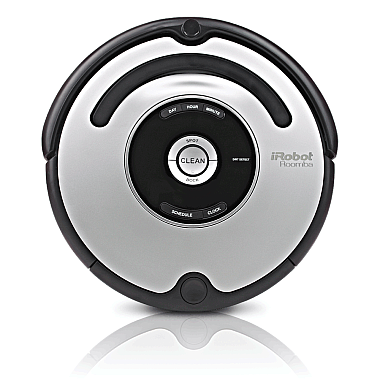
\includegraphics[width=0.3\textwidth]{images/roomba}}
	~
	\subfloat[A Samsung Galaxy S II]{\includegraphics[width=0.3\textwidth]{images/Samsung}}
	~
	\subfloat[An XBOX 360 controller]{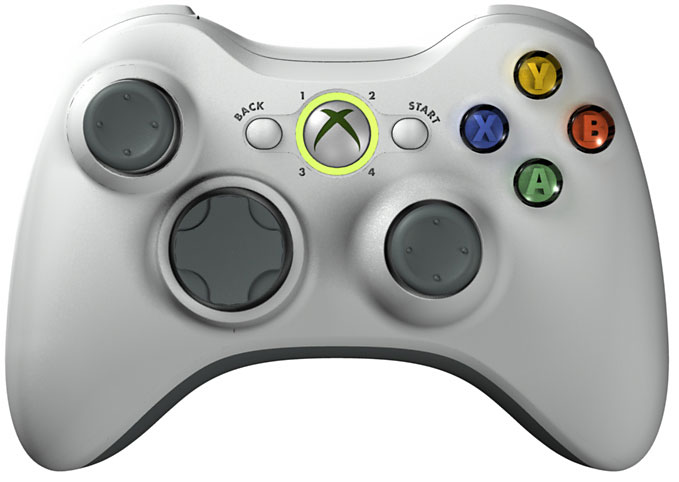
\includegraphics[width=0.3\textwidth]{images/xbox-360}}
	\caption{The hardware used in the study, a Roomba vacuum cleaner, a Samsung Galaxy S II, and an XBOX 360 controller.}
	\label{hardware}
\end{figure}

\section{XBOX 360 Controller}
The XBOX 360 controls for the Roomba are written in Python (see Appendix). The program uses a library called RoombaSCI to communicate with the Roomba via Bluetooth. RoombaSCI is a Python wrapper for iRobot's Serial Command Interface Specification, which allows commands to be sent to the Roomba through its serial port. RoombaSCI abstracts tasks like setting up the connection and sending bytes to specific motors into commands like \texttt{FORWARD}, \texttt{STOP}, and \texttt{SPIN LEFT} \cite{RoombaSCI}. It also allows the programmer to set the speed of the Roomba within the range allowed by the hardware (-500 - 500 mm/s). \cite{iRobot}

A RooTooth bluetooth-serial adapter was used to communicate with the computer wirelessly. The Pygame library is also used to properly capture the input from the controller. 

The end result is a controller that can be used to move forward/backward and rotate to the left or right in place. The right trigger sends the \texttt{FORWARD} command, the left trigger sends \texttt{BACKWARD}, and the left analog stick pressed to the left or right sends a \texttt{LEFT} or \texttt{RIGHT} command (see Figure~\ref{xbox_diagram}). The robot continues moving forward/backward/left/right as long as the trigger or analog stick is held, and will stop when it is released, or another button is pressed. When using the XBOX 360 controller, the robot can only move at the maximum speed, and it can only perform one of forward/backward or rotation at any given time (forward motion must stop in order to turn). The left and right controls are not gradual, meaning that leaning the analog stick partially to the side does nothing. In order to turn left/right, the analog stick must be pushed completely to one side or the other.

\begin{figure}[h!]
	\centering
	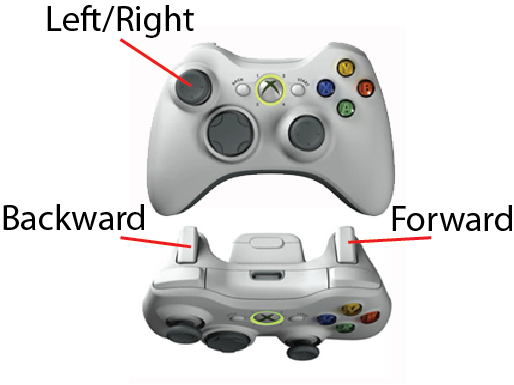
\includegraphics[scale=0.4]{images/xbox_diagram}
	\caption{The XBOX 360 control scheme. The left analog stick controls left and right turns, while the triggers control forward and backward movement.}
	\label{xbox_diagram}
\end{figure}

\section{Cellbots Application}
The D-Pad and the tilt controls were downloaded to the phone as part of a single app called Cellbots. Cellbots is an open source Android application, available for free online or in the Android Market. The app comes with four control schemes, including the D-Pad controls and the tilt controls (Figure~\ref{cellbots}). It also included voice controls and an on-screen Atari-style joystick which were not used in the experiments but could be utilized in future research.

\begin{figure}
	\centering
	\subfloat[The D-Pad controls. Each of the four directional buttons cause the robot to move.]{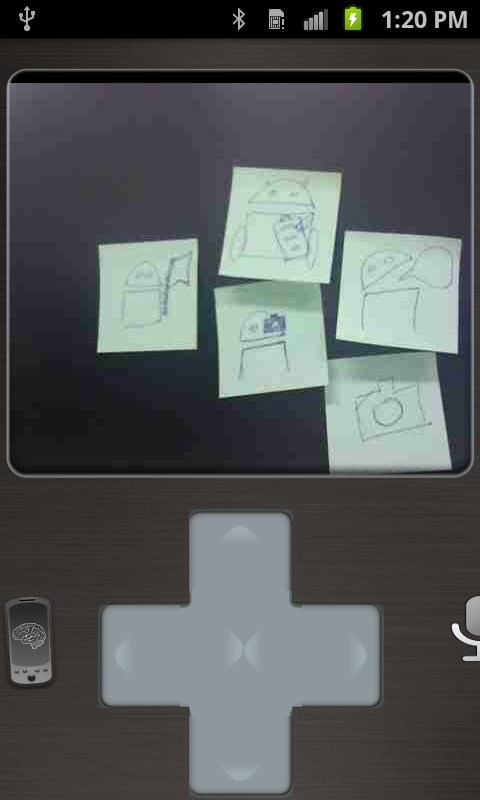
\includegraphics[scale=0.3]{images/dpad}}
	~
	\subfloat[The tilt controls. Holding the center button and tilting the phone causes the robot to move.]{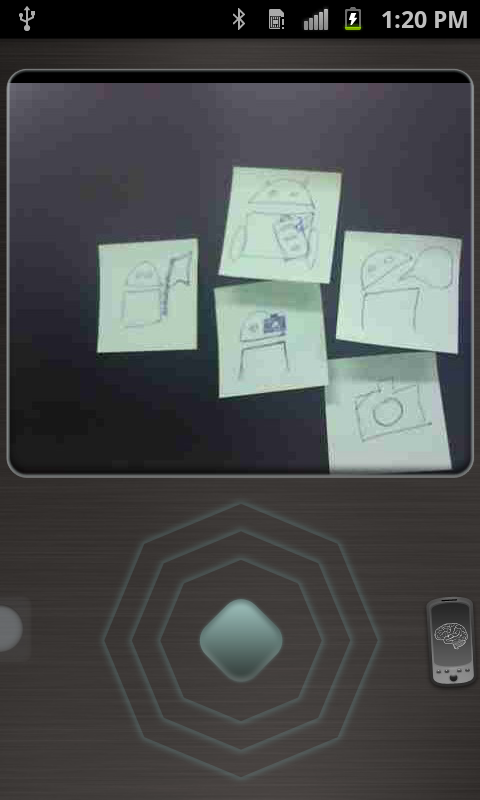
\includegraphics[scale=0.3]{images/tilt}}
	\caption{Two of the screens from Cellbots, D-Pad and tilt.}
	\label{cellbots}
\end{figure}

The D-Pad controls require the user to press one of four on-screen buttons, arranged in a cross. Like the XBOX 360 controller, the robot moves forward/backward and rotates in place when the appropriate button is held down, stopping when the button is released. Also like the XBOX 360 controller, the D-Pad only allows one speed and one type of movement at a time.

The tilt controls use the phone's accelerometers to control the robot. The user holds the phone horizontally (screen facing up) and holds down an on-screen button. While the button is held down, tilting the phone forward (rotation around its x-axis) causes the robot to begin to drive forward. The phone can be rolled right or left (rotating around its y-axis) to steer. Figure~\ref{acceleration_axes} shows the phone's axes.

\begin{figure}[h]
	\centering
	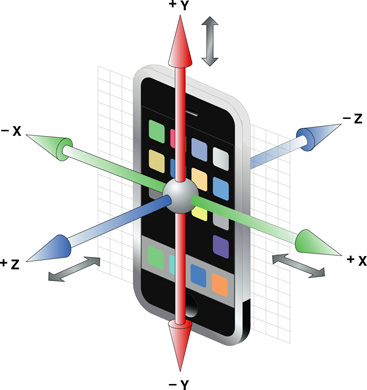
\includegraphics[scale=0.5]{images/acceleration_axes}
	\caption{The smartphone's x, y, and z axes.}
	\label{acceleration_axes} 
\end{figure}

The tilt controls differ from the other controls in two ways: first, the speed can vary. The more the phone is tilted forward, the faster the robot moves, up to the maximum speed of 500 mm/s.  The second difference is that the tilt controls allow forward/backward motion and turning at the same time. For example, if the phone is tilted forward and rolled left, the robot will perform a left turn, rather than rotating in place.

\section{Gesture-Based Control Application}
The gesture-based controls are implemented on top of the existing Cellbots application. Cellbots is an open source application, so the gesture controls were added as a fifth control type. 

To recognize the gestures using accelerometers only, I turned to another open source Android application called GestureTrainer. GestureTrainer is an implementation of the concepts outlined in \cite{TaKG} for gesture recognition using accelerometer data.

\begin{figure}[h]
	\centering
	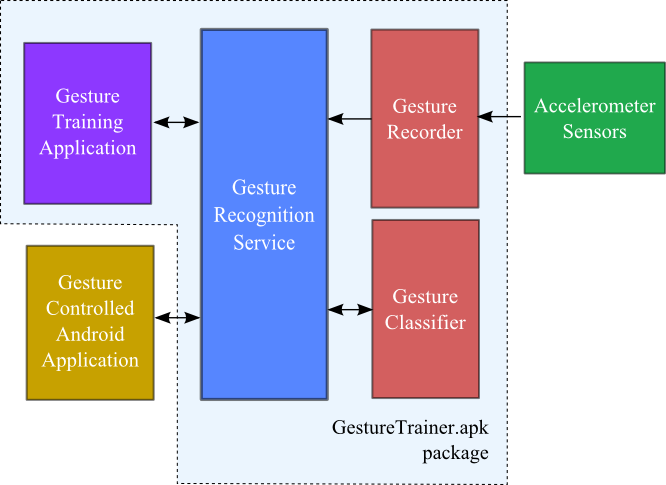
\includegraphics[width=\textwidth]{images/gesture_framework}
	\caption{The GestureTrainer architecture. The Cellbots app was modified to include Gesture Recognition Service, Gesture Recorder, and Gesture Classifier, making it a Gesture Controlled Android Application}
	\label{gesture_framework}
\end{figure}

Users can record and name their own gestures on the phone, and from then on when the gesture is performed and recognized, the name is sent to the Roomba. The phone recognizes gestures continuously, without the need to specify when the user is about to perform a gesture.

To record a gesture, the user presses a button to start ``learning mode". The phone receives a constant stream of events for every movement that the accelerometer picks up in the form of a vector of floats, ($\Delta x, \Delta y, \Delta z$). If the norm of the vector is above a certain threshold, the movement is considered ``significant" and the app begins recording the stream of vectors. When the phone receives 10 events in a row whose norms do not exceed the threshold, the gesture is determined to be complete. The list of xyz-vectors is stored as a Gesture object, and given the name specified by the user. 

After exiting ``learning mode", the phone begins recognizing gestures immediately. When a gesture is detected, it is stored in a Gesture object, and sampled by one of several different feature extractors. The feature extractors serve to divide the gesture into a certain number of vectors, or normalize the values in the vectors. We then compute the distance between this sampled signal and each of the user's recorded gestures.

The distance calculation from Gesture $a$ to Gesture $b$ is done through the Dynamic Time Warping algorithm (see Appendix for source code). A $a.length \times b.length$ matrix of floats, $dist$, is constructed, where entry $dist(i,j)$ is the norm of the $i$th vector in $a$ minus the $j$th vector in $b$. A second matrix of the same size, $cost$, is constructed so that the first column of $cost$ is the same as the first column of $dist$, and the rest of the entries are 0.

The $cost$ matrix is filled in dynamically from the top left ($cost(0, 0)$) to the bottom right ($cost(a.length, b.length)$), iterating over columns first, then rows. To compute $cost(i, j)$, the current minimum cost is computed as \[minCost = cost(i - 1, j - 1) + dist(i, j)\] This is the value assigned to $cost(i, j)$. If $cost(i - 1, j) + dist(i, j) < minCost$ or $cost(i, j - 1) + dist(i, j) < minCost$, an additional offset penalty of 0.5 is added to $cost(i, j)$.

After the whole $cost$ matrix has been filled in, the entry $cost(a.length - 1, b.length - 1)$ (the bottom right corner), is the minimum distance between the two Gestures $a$ and $b$. The stored Gesture with the smallest distance from the performed Gesture is the one that is selected to be sent to the Roomba. The last step is to check that distance against a threshold. If the distance is less than the threshold, then the command would be sent, otherwise no command is sent. This is to ensure that all commands sent were close matches, since every gesture will return a match with some stored gesture, even if there are no similar gestures. If the closest match has a high distance, it is not close enough to be executed as a command so it is ignored.

\begin{figure}[h!]
	\centering
	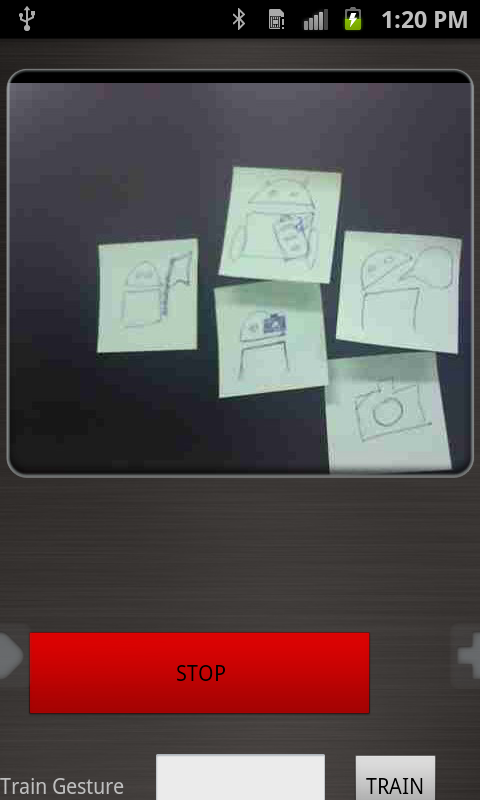
\includegraphics[scale=0.2]{images/gesture}
	\caption{The gesture-based controller screen added to Cellbots. It uses the code and algorithms from GestureTrainer to perform gesture recognition, and also has a \texttt{STOP} button.}
	\label{gesture_cellbots}
\end{figure}


One of the major benefits of using this algorithm is that the gesture recognition is performed with only one sample. Other gesture recognition systems, like the one outlined in \cite{Rubine} require multiple samples to perform recognition reliably.

This code was integrated into Cellbots as another control view, to ensure that the same speeds/timing would be used for each control scheme on the phone  (Figure~\ref{gesture_cellbots}).

The gestures defined were \texttt{FORWARD}, \texttt{BACKWARD}, \texttt{LEFT}, and \texttt{RIGHT} (see Figure~\ref{gesture_photos} for demonstrations of each gesture). 

\begin{figure}[h!]
	\centering
	\subfloat[\texttt{FORWARD} gesture (high to low).]{\reflectbox{%
	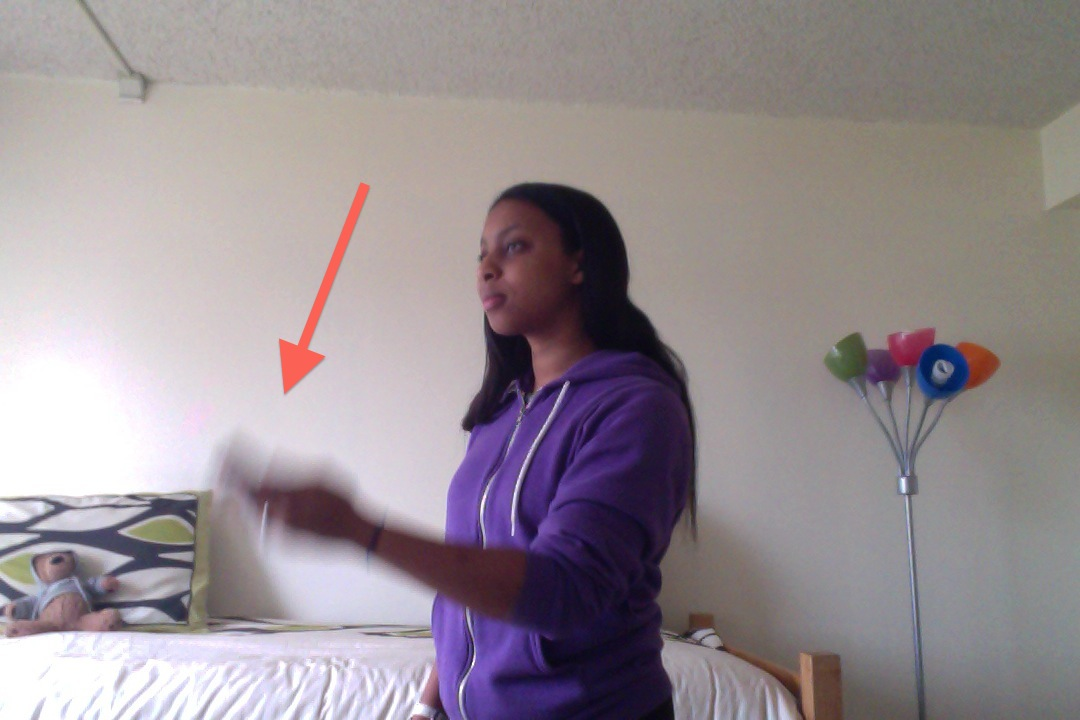
\includegraphics[width=0.5\textwidth]{images/forward}}}
	~
	\subfloat[\texttt{BACKWARD} gesture (two counterclockwise circles).]{\reflectbox{%
	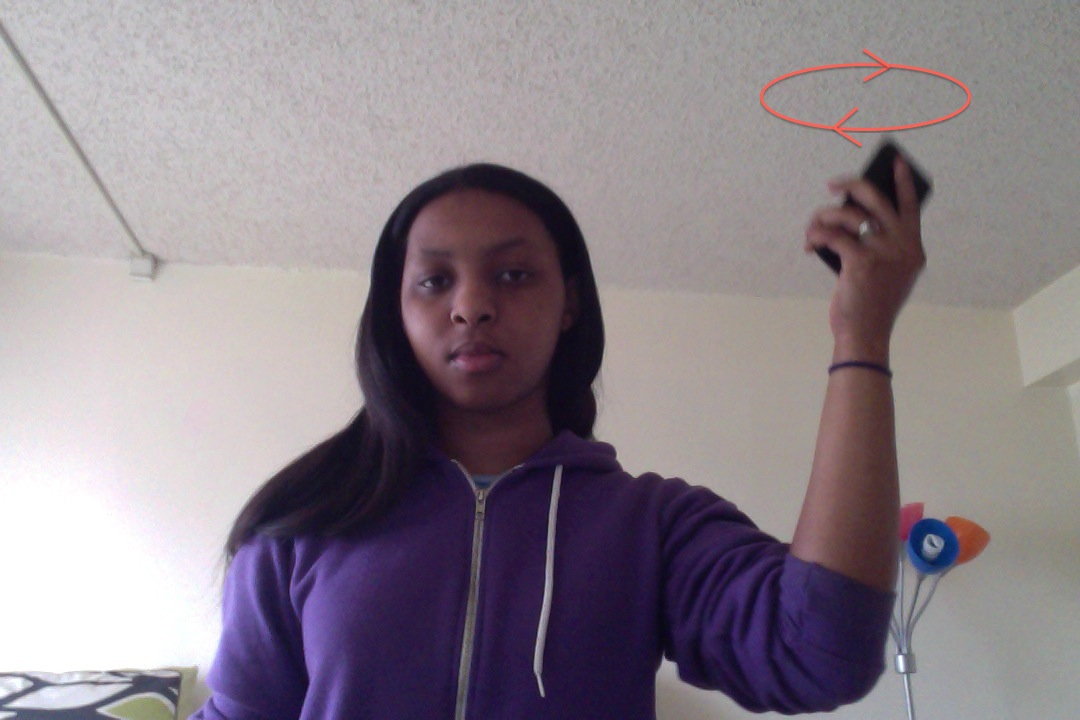
\includegraphics[width=0.5\textwidth]{images/backward}}}
	
	\subfloat[\texttt{LEFT} gesture (right to left).]{\reflectbox{%
	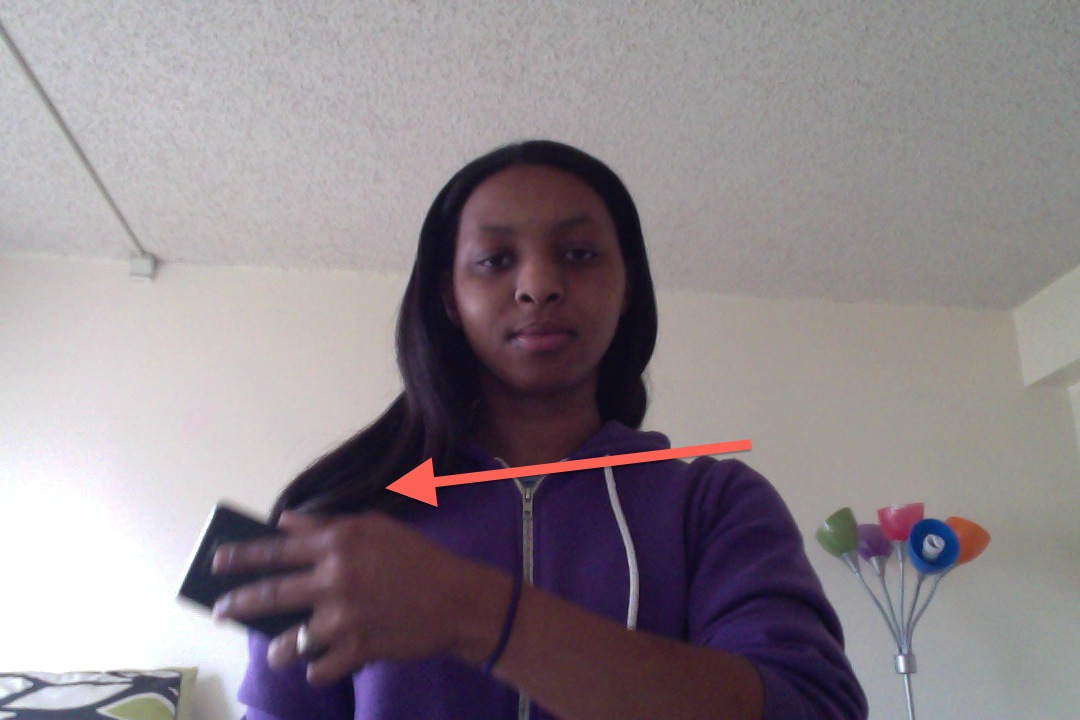
\includegraphics[width=0.5\textwidth]{images/left}}}
	~
	\subfloat[\texttt{RIGHT} gesture (left to right).]{\reflectbox{%
	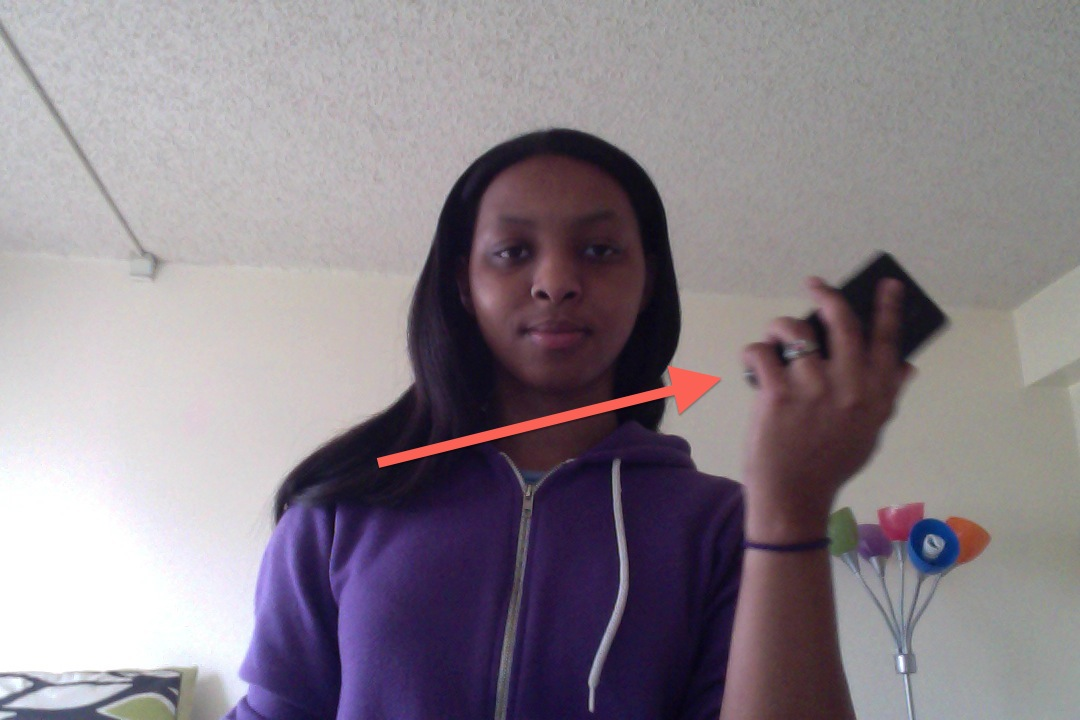
\includegraphics[width=0.5\textwidth]{images/right}}}
	
	\caption{The four gestures defined in the gesture-based application.}
	\label{gesture_photos}
\end{figure}

All the gestures are performed with the phone's screen facing the user. The \texttt{STOP} command was left as an on-screen button, rather than a gesture, to make it easier for the subject to maintain control (and for the sake of the hardware and testing environment).

\chapter{Human Factors Experiment Design}
In this chapter I will describe the setup of the human factors experiment, as well as the design choices. The human factors experiment was conducted with 15 subjects to gauge the effectiveness of each controller. The experiment involved empirical metrics (such as time taken to complete course and number of times the robot crossed the boundaries), as well as qualitative data obtained through a questionnaire.
\section{Platform and Hardware}
The Roomba was chosen because it is a commercial, off the shelf robot that is relatively easy to control via a store bought Bluetooth adapter. It has two motorized wheels in the center and a single caster in the front for smooth forward steering. The lack of a back caster meant that the Roomba's backwards movement could sometimes become slightly erratic at maximum speed, but for the most part, the movement was unaffected.

The Samsung Galaxy S II was chosen primarily for its gyroscopes. All Android phones come with accelerometers, but only some with gyroscopes, which help the phone to give more precise measurements. The Microsoft XBOX 360 controller was chosen because until recent games like ``Mario Kart Wii", most driving/navigating games are were made for the XBOX 360, making its controller a good ``standard" controller.
\section{Track Design}
The track used in the experiments is based on a beginner's time trial circuit from Nintendo's ``Mario Kart Wii" called Mario Circuit (sometimes Mario Raceway). 

\begin{figure}
	\centering
	\subfloat[Mario Circuit, as seen in the video game ``Mario Kart Wii".]{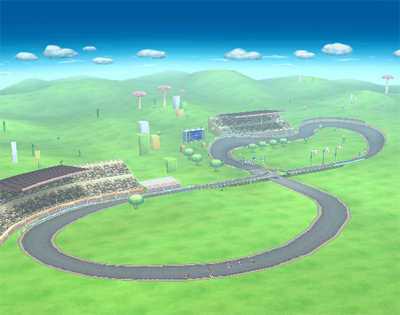
\includegraphics[width=0.5\textwidth]{images/mario_circuit_screenshot}}
	~
	\subfloat[The original floor plan for the course used in the study. It was later scaled to be appropriate for the size of the Roomba and the lab space in which the experiment took place.]{
\includegraphics[width=0.5\textwidth]{images/MarioCircuitLayout}}
	\caption{Comparison of the original Mario Circuit track with the course used in the experiments.}
	\label{mario_circuit}
\end{figure}

The course used in the study is a scaled down version of Mario Circuit, which is a slight variation on a traditional figure-eight course (see Figure~\ref{mario_circuit}). The course was chosen primarily because it involves two U-turns (one left, and one right), a left turn, a right turn, and two straightaways, allowing all the commands to be tested every lap. In the game, players race around the track for 3 laps, and the 3 lap requirement was kept for the experiment. Subjects completed 3 laps, then crossed the finish line a few yards away. A ``Mario Kart Wii" course was also chosen because ``Mario Kart Wii" is the  best-selling racing game of all time, and Mario Circuit is an updated version of one of the classic courses, originally created by the game designers as the premier time trial course \cite{MarioCircuit}. 

\section{Questionnaire Design}
The questionnaire opens with basic demographic questions (age, gender, field of study/profession, etc.), then   asks about subjects' video game habits and computer experience. The questionnaire then asks the following specific questions about each of the four controllers (on a five-level Likert scale unless otherwise specified):
\begin{itemize}
\item How aware were you of the controls while you were using them?
\item How awkward was holding the controller in your hand?
\item Did you feel that you were fully in control of the robot at all times? (Yes/No)
\item How difficult was it to maintain control while driving in a straight line? 
\item How difficult was it to maintain control while turning?
\item How difficult was it to learn the controls?
\item Did you perform as well as you wanted to in the obstacle course? (Yes/No)
\item What was your favorite part about this control scheme? (Short Answer)
\item What was your least favorite part about this control scheme? (Short Answer)
\end{itemize} 
Finally, the questionnaire asks participants to rank controllers according to which they would use to accomplish a critical task, which they would use continuously for two hours, which was most intuitive, and which was most fun.

\section{Experiment Procedure}
When subjects arrived, they were first briefed on the purpose of the experiments. Every subject tried the controllers in a randomized order. A short period was allowed for the subject to get used to the controller before beginning the time trial course. The subject completed three timed laps around the course. Subjects were allowed to move between several locations outside the track during a run of the course, but were not allowed to touch the robot or follow it closely. The number of times the robot went outside the boundaries was recorded, along with the number of ``mistake acknowledgements". I defined ``mistake acknowledgements" as a physical or verbal cue that the subject performed a command they did not intend. Examples of mistake acknowledgements include stamping one's foot, shaking one's head, statements like ``No" and ``Oops", and swearing. After every run, the subject was informed of his/her time with that controller. Immediately after all four of the time trials were finished, the subject filled out the questionnaire. 

\chapter{Results}
In this chapter I will present the results of the experiments and questionnaire. First, a breakdown of the empirical data from the time trials is given, followed by the data from the questionnaire. Finally, I provide my analysis of both sets of data and present some hypotheses based on the combined data.

\section{Time Trials}
For the time trials, I recorded the time of each lap, the total time taken to complete the course, the number of ``line faults" (robot crossing out of the boundaries), and ``mistake acknowledgements" (defined in Section 4.4). The averages for each of these values are presented in Table~\ref{averages}. It should be noted that there were several subjects with times more than 2 standard deviations from the mean (3 in some cases). Because of the small sample size, their data was not excluded from the calculations. The full raw data can be found in the Appendix.

\begin{table}[h]
	\begin{tabular}{|c||l|l|l|}
	\hline 
	Controller & Avg. Time (sec) & Avg. Line Faults & Avg. Mistake Ack. \\ 
	\hline 
	D-Pad & 161.53 & 0.07 & 0.4 \\ 
	\hline 
	Tilt & 164.58 & 2.13 & 2.6 \\ 
	\hline 
	Gesture & 393.81 & 6.67 & 7.0 \\ 
	\hline 
	XBOX 360 & 124.74 & 0.93 & 0.5 \\ 
	\hline 
	\end{tabular} 
	\caption{Average time taken to complete the course, average number of Line Faults, and average number of Mistake Acknowledgements for each of the four controller types.}
	\label{averages}
\end{table}

The XBOX 360 controller had the fastest average time, with 124.74s, while the D-Pad and Tilt controllers were both approximately equal (161.53s and 164.58s, respectively). The gesture-based controls performed the slowest, with an average time of 393.81s.

Though the XBOX 360 controller had the fastest average time, the fastest individual time belonged to the tilt controller: one subject completed the course in 83.3s, making the tilt controller the only controller with a total time under 100s.

The D-Pad averaged the fewest line faults by far, with 0.07 (there was a total of 1 line fault across all subjects), while the gesture-based controls again came in last with an average of 6.67 faults.

The D-Pad also averaged the fewest mistake acknowledgements, with 0.4 average mistake acknowledgements. The XBOX 360 controller was just behind the D-Pad with an average of 0.5 mistake acknowledgements. The gesture-based controls averaged 7.0 mistake acknowledgements, more than 17 times the average number of mistakes acknowledged with the D-Pad. The gesture-based system was also the only one where the minimum number of mistake acknowledgements was above 0; every single subject acknowledged at least one mistake.

\section{Questionnaire}
Presented here are answers to several relevant questions. More data can be found in the Appendix.

The D-Pad receieved mostly positive reviews, though 60\% of respondents said that they were aware of the controls while using them. 80\% said the controller was not awkward, and that they felt that they were fully in control of the robot at all times. 100\% of respondents rated the controls as easy to learn. 80\% said that they performed as well as they wanted to in the course. Many subjects enjoyed the ``simplicity" and ``familiarity" of the D-Pad, along with the fact that the directional arrows were visible. The most popular complaint about the D-Pad was that it could only handle one command at a time and could not turn and move simultaneously. It was also described as ``mundane" and ``less fun than [some other controls]".

In a slight jump up from the D-Pad, 66\% of subjects said they were aware of the tilt controls while using them. 53\% rated the controls awkward, and only 60\% said they felt in control of the robot at all times. 40\% of respondents said they performed as well as they wanted to (a large deviation from the D-Pad). Subjects praised the tilt controls for being ``intuitive", ``smooth", and ``fun", while others criticized it for being ``hard to control".

The gesture-based controls did not fare as well. 80\% of users said that they were aware of the controls while using them, and 66\% described them as awkward. 86.7\% of subjects said they did not feel in control of the robot at all times, and 86.6\% said it was difficult to maintain control while turning (46\% rated it hard to control while driving in a straight line). The majority of subjects rated the gestures somewhat easy to learn. Subjects enjoyed the ``novelty" of the gesture-based controls, but ultimately decided it was ``unresponsive", ``inaccurate", and ``frustrating" at times.

The XBOX 360 controller got slightly better ratings than the gesture-based controls. Most respondents said that they were somewhat aware of the controls, while 86.6\% rated it not awkward. 86.7\% said they felt that they were fully in control of the robot at all times, which is the most of all the controllers. 100\% rated the XBOX 360 controller easy to learn. 86.7\% performed as well as that wanted to in the course. Subjects praised it for being ``familiar", ``easy to learn", and for having a physicality that allowed them to keep their eyes on the robot at all times. There were, however, many complaints about not being able to turn while moving forward, like the tilt controls, and having no way to gradually increase the amount the robot was turning. 

\begin{figure}[h!]
	\centering
	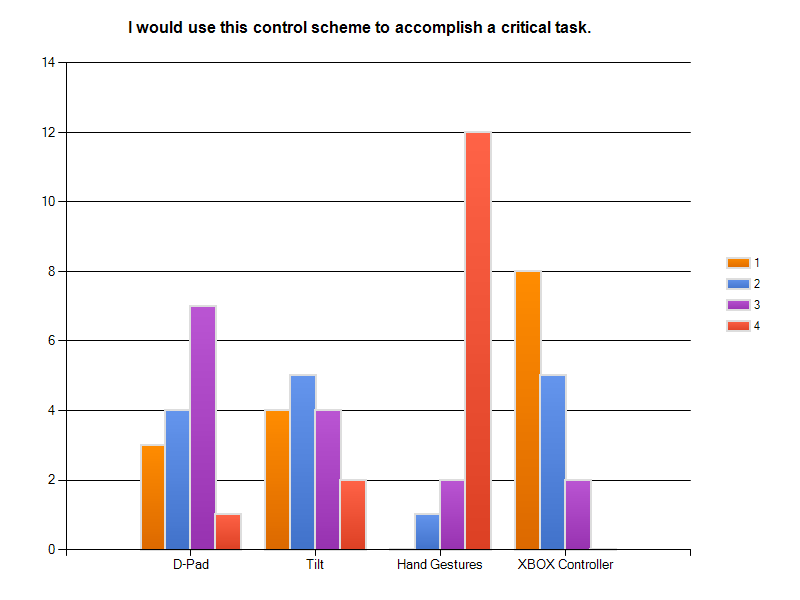
\includegraphics[width=4.5in]{images/sm_50.png}
	\caption{The numbers 1-4 indicate rank given to the controller for using it to accomplish a critical task. The XBOX 360 controller was the most popular for accomplishing a critical task; the gesture-based controls were the least popular.}
	\label{sm_50}
\end{figure}

The majority of subjects, 53.3\% said that they would use the XBOX 360 controller as their first choice for accomplishing a critical task. 80\% of subjects ranked the gesture-based controls last for accomplishing a critical task, with no users ranking it as their first choice (see Figure~\ref{sm_50}).

Similarly, 71\% of subjects would use the XBOX 360 controller for two hours continuously, while 80\% ranked the gesture-based controls in last place (see Figure~\ref{sm_51}).

\begin{figure}[h!]
	\centering
	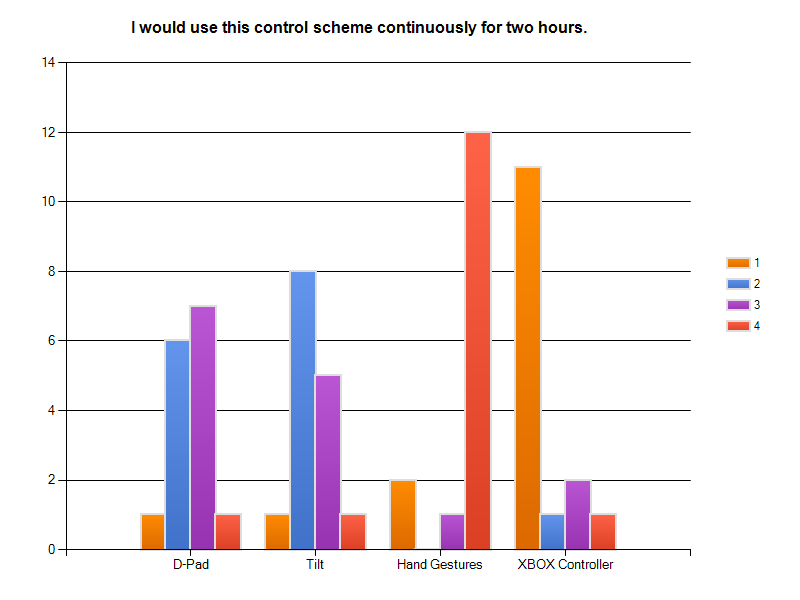
\includegraphics[width=4.5in]{images/sm_51.png}
	\caption{The numbers 1-4 indicate rank given to the controller for using it for two hours continuously. The XBOX 360 controller was the most popular for using continuously for two hours; the gesture-based controls were the least popular.}
	\label{sm_51}
\end{figure}

The tilt controller was ranked the most intuitive (40\%), followed by the D-Pad, then the XBOX 360 controller. No subjects rated the gesture-based controls the most intuitive (see Figure~\ref{sm_52}).

\begin{figure}[h!]
	\centering
	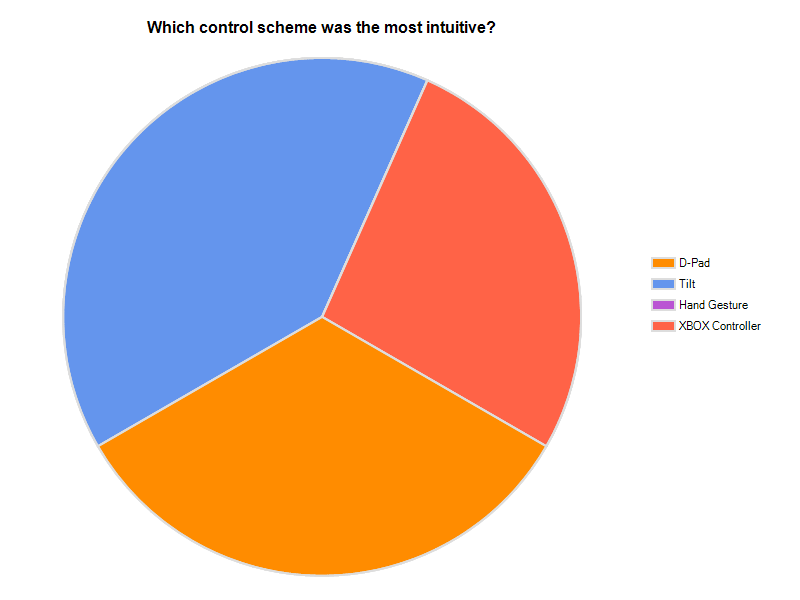
\includegraphics[width=4.5in]{images/sm_52.png}
	\caption{The tilt controller was ranked the most intuitive, while the gesture-based controller was ranked the least intuitive.}
	\label{sm_52}
\end{figure}

The tilt controller was also ranked the most fun to use, followed by the XBOX 360 controller, with D-Pad and gesture-based tying for third (see Figure~\ref{sm_53}).

\begin{figure}[h!]
	\centering
	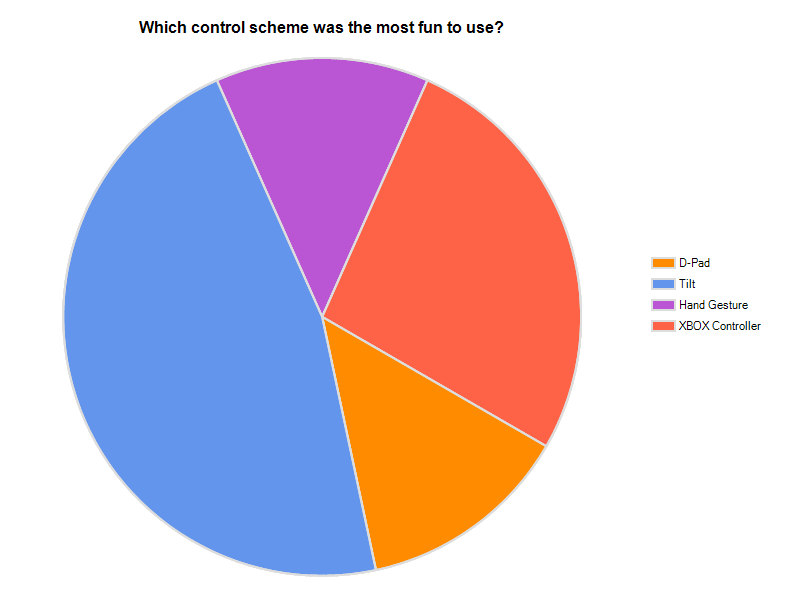
\includegraphics[width=4.5in]{images/sm_53.png}
	\caption{The tilt controller was ranked the most fun to use, while the D-Pad and gesture-based controls tied for 3rd place.}
	\label{sm_53}
\end{figure}

\section{Analysis and Hypotheses}
Empirical data shows that the XBOX 360 controller was the fastest, and the second most ``error free", meaning a low number of line faults and mistake acknowledgement. The gesture-based controls performed poorly, with an average time, average number of faults, and average mistake acknowledgement more than twice that of all the others controllers. The qualitative data also showed that the gesture-based controls were not well suited to the task. 

Based on these two sets of data, I believe that the gesture-based controller is not a good system for direct control of a vehicle.

One major problem with the gesture-based controls is the timing. In order to recognize a gesture, the gesture must be fully completed. This means that when a subject wants to issue a command, he/she must complete the entire movement before the phone can classify the gesture and send it to the robot. Compare this to pressing a button, which is almost instant. There is no recognition process with a button press, so as soon as the button is fully pressed, the command can be sent to the robot. Many subjects felt frustrated waiting for the entire gesture to finish and be classified before the command was sent. Often, subjects tried to make up for the lost time by gesturing faster/more firmly, but this would often cause unwanted accelerometer data which led to incorrect classifications.

This could be remedied in part by using a system more like the one usually used with the Microsoft Kinect. Rather than gestures, most of the commands are given through positioning of the hands/body. Using the position of the hand, a system could be constructed that allows for faster recognition, along with gradual turning and speed changes, rather than sending a string of commands.

The other major problem with the gesture-based controls was accuracy. Gestures can be recognized incorrectly, whereas buttons cannot provide incorrect information (a user could accidentally press the wrong button, but a properly working set of buttons will always send the right information). The fact that gestures do not have 100\% accuracy adds a layer of computer error on top of the possible human error, which can be very dangerous.

The emotions of the user also come into play with gesture-based controls in a way that they do not with buttons or tilt based controls. A calm user will gesture a certain way, while an agitated user will usually gesture more wildly. A wild gesture's accelerometer data is much more likely to appear different from the original gesture's data, making it more likely to be classified incorrectly. This is amplified into a negative feedback cycle when a user makes a mistake, because often the user will gesture more vehemently to correct the mistake, leading to more mistakes. Buttons and tilt-based controllers are not affected by how frantic or agitated the user is. 

This is not to say that gesture-based controls have no place in robotics, but that they would most likely be better suited for a higher-level set of commands. Gesture-based controls were originally explored because gestures are a natural human form of communication, but when humans gesture, it is very rarely to communicate low level directions like ``go forward", ``stop, and ``rotate left". More often the commands assume a certain level of autonomy on the part of the receiver. For example, telling another person ``join me" through a hand gesture assumes that the person will figure out how to navigate the room on his own. Many subjects said that they felt that the gesture-based controls were ``unintuitive" (no subject ranked it as the most intuitive) ``frustrating", and ``tiring". I believe it is because the commands being sent were too low-level for the gesture-based controls used in the study to be effective. 

Gestures used between humans also rely on the fact that the receiver can see/calculate where the other person is indicating. Many human gestures for navigation correspond to phrases with an explicit point of reference (ex. ``follow me", ``go over there"). The Army Field Manual details many such gestures \cite{VisualSignals}. Using gestures to control the robot's direct movement was therefore somewhat unintuitive to subjects who were not used to applying a high-level form of communication to a low-level command. 53.3\% of the subjects improved over the three laps, which indicates that the gesture-based controls used in the study may require more training time, not less as was originally thought.

\chapter{Conclusion}
In this thesis, I presented a suite of robotic control systems: an XBOX 360 controller, a touchscreen D-Pad, a tilt controller, and a hand gesture controller. All systems were composed of commercial, off the shelf hardware. A study with empirical and qualitative data was conducted to determine the most effective of the controllers. The empirical data showed the XBOX 360 controller to be the most effective (fastest), and the D-Pad to be the least error prone. By contrast, the gesture-based controls were shown to be both the slowest and the most error prone. The qualitative data showed that the gesture controls were thought to be the least intuitive and one of the least enjoyable controllers to use, while the tilt controller was ranked the most intuitive and the most enjoyable. 

Based on the data and analysis, gesture-based controls should continue to be explored, but the focus should shift to the context of more autonomous robots who can safely navigate their own environment. It appears that most of the problems that subjects had with the gesture-based controls could be alleviated by implementing a different set/style of commands. Results for gesture-based controllers could perhaps be improved by allowing the subject to define his/her own gestures, or implementing more tilt style controls using accelerometer data combined with computer vision data.

\bibliographystyle{plain}
\bibliography{rough}

\clearpage
\pagestyle{plain}
\chapter*{Appendix}
\section*{Gesture Recognition Code}
This is the portion of the GestureTrainer/Cellbots code that calculates the distance between two Gestures, $a$ and $b$. The Gesture class is essentially an object wrapper for \texttt{String label},which represents the Gesture's name, and \texttt{List<float[]> values}, which represents the stream of $(x, y, z)$ values recorded.
\lstset{language=Java, breaklines=true, tabsize=2}
\lstinputlisting{DTWAlgorithm.java}

\section*{Time Trials Raw Data}

\section*{Questionnaire Data}
%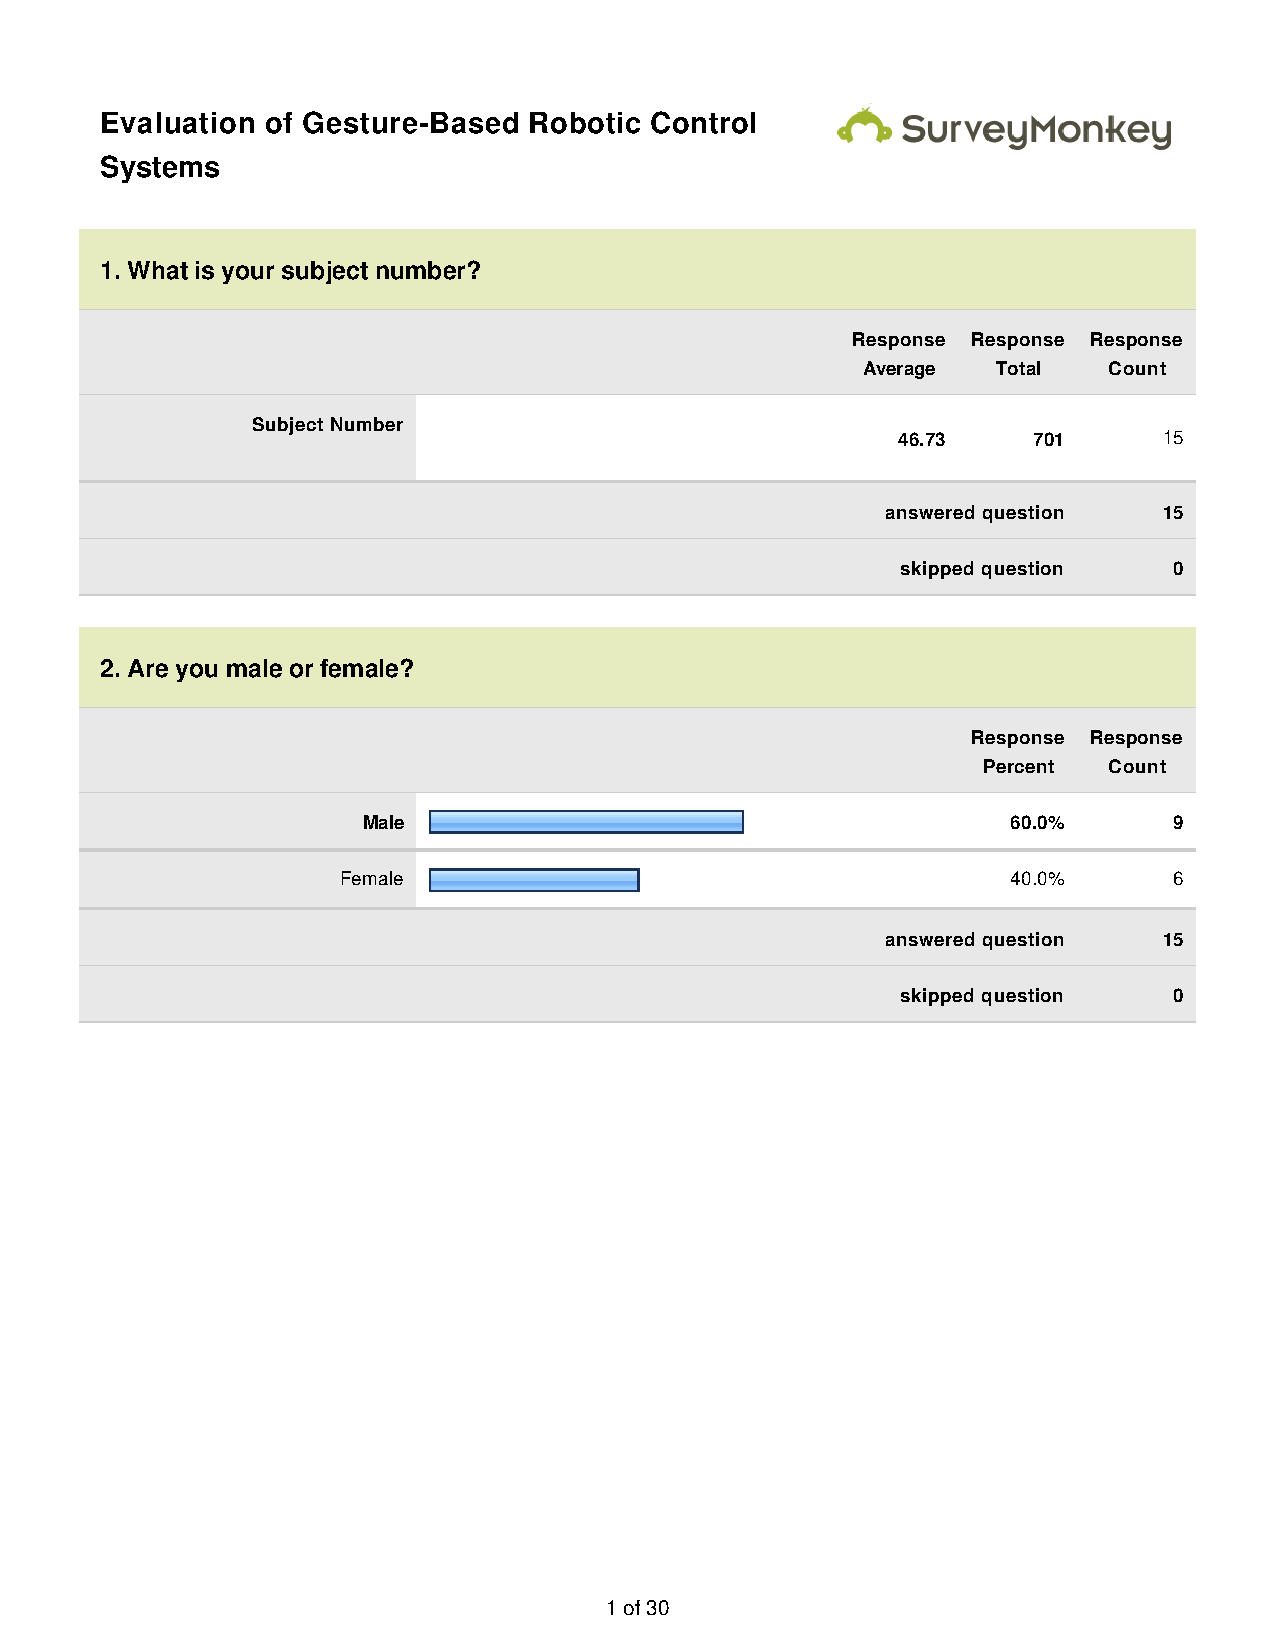
\includepdf{Questionnaire.pdf}
\end{document}